\lecture{20}{7 maggio 2024}
\section{Riflessione e rifrazione}
Consideriamo ora il caso di un'onda elettromagnetica che viaggia in un mezzo con una certa impedenza e che incontra un altro mezzo con impedenza diversa. È diverso dal caso su una corda, banalmente perché stiamo lavorando con equazioni alle derivate prime (equazioni di Maxwell). Consideriamo un caso molto semplice con un'onda elettromagnetica monocromatica polarizzata linearmente, due mezzi omogenei (impedenze \(Z_1, Z_2\)), una superficie di separazione piana tra i due mezzi, l'onda che incide perpendicolarmente rispetto alla superficie (incidenza normale).
\begin{figure}[H]
	\centering
	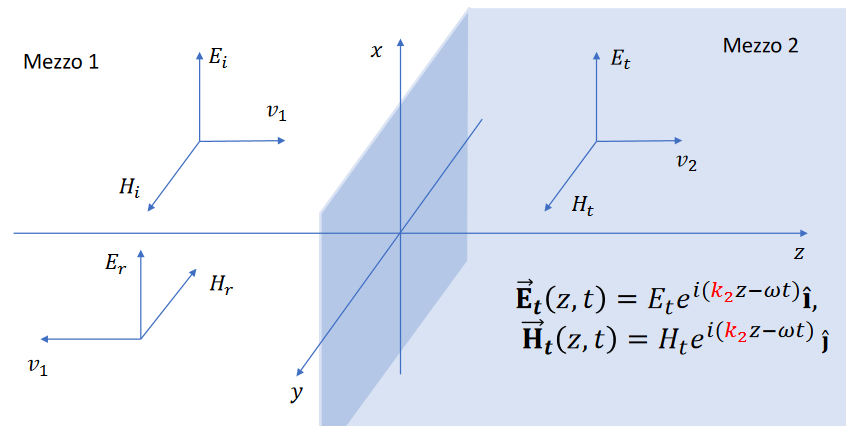
\includegraphics[width=0.5\textwidth]{screenshots/2024-05-07-11-22-20.png}
\end{figure}
Le onde incidenti sono \(\vec{E}_i(z,t)=E_i e^{i(k_1 z- \omega t)}\vec{\hat{i}}\) e \(\vec{H}_i(z,t)=H_i e^{i(k_1 z -\omega t)}\vec{\hat{j}}\). Si avranno onde riflesse:
\begin{align}
	\vec{E}_r(z,t) &= E_r e^{i(-k_1 z - \omega t)} \vec{\hat{i}} &
	\vec{H}_r(z,t) &= - H_r e^{i(-k_1 z - \omega t)} \vec{\hat{j}}
\end{align}
dove il segno di \(H_r\) è negativo per avere una terna destrorsa. Si hanno anche onde trasmesse:
\begin{align}
	\vec{E}_t(z,t)&=E_t e^{i(k_2 z -\omega t)} \vec{\hat{i}} &
	\vec{H}_t (z,t)&=H_t e^{i(k_2 z- \omega t)} \vec{\hat{j}}
\end{align}
Ricordo la relazione che sussiste fra \(\vec{H}\) e \(\vec{E}\) nelle onde elettromagnetiche:
\begin{gather}
	\vec{H} = \frac{\vec{k}}{\omega \mu } \cp \vec{E}\\
	\implies \vert \vec{H} \vert = \frac{\vert \vec{E} \vert }{Z}
\end{gather}
Le impedenze dipendono dall'impedenza del vuoto attraverso l'inverso dell'indice di rifrazione: \(Z_1 = \quotient{Z_0}{n_1}\) e \(Z_2 = \quotient{Z_0}{n_2} \).
Di conseguenza i moduli di \(\vec{H}\) ed \(\vec{E}\) possono essere collegati così:
\begin{align}
	H_i &= n_1 \frac{E_i}{Z_0} &
	H_r &= n_1 \frac{E_r}{Z_0} &
	H_t &= n_2 \frac{E_t}{Z_0}
\end{align}
Dobbiamo ora trovare le relazioni fra i campi elettrici.
\begin{figure}[H]
	\centering
	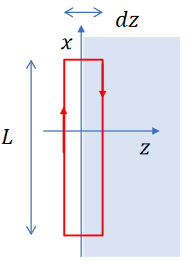
\includegraphics[width=0.3\textwidth]{screenshots/2024-05-07-11-32-18.png}
\end{figure}
Attraverso la curva rappresentata nella figura il flusso del campo magnetico tende a zero (l'area tende a zero), quindi la circuitazione del campo elettrico è nulla. Il contributo dei due lati piccoli tende a zero se i lati tendono a zero. Da questo segue che
\begin{equation}
	E_i + E_r = E_t
\end{equation}
Facciamo lo stesso ragionamento per il campo \(\vec{H}\). Non ci sono correnti concatenate e il flusso del campo elettrico attraverso la superficie tende a zero. Da questo segue che la circuitazione del campo \(\vec{H}\) è nulla, quindi
\begin{equation}
	H_i - H_r = H_t
\end{equation}
Il segno negativo davanti ad \(H_r\) deriva dal fatto che \(\vec{H}\) riflesso è opposto rispetto ad \(\vec{H}\) incidente.
Ho trovato un sistema di equazioni che mi permette di esplicitare i campi trasmessi e riflessi rispetto al campo incidente.
\begin{gather}
	\begin{cases}
		E_i +E_r = E_t\\
		n_1 \frac{E_i}{Z_0} - n_1 \frac{E_r}{Z_0} = n_2 \frac{E_t}{Z_0}
	\end{cases}
	\implies 
	\begin{cases}
		E_t = E_i + E_r\\
		n_1 E_i - n_1 E_r = n_2 E_i + n_2 E_r
	\end{cases}\\
	\implies 
	\begin{cases}
		E_t = \frac{2n_1}{n_1 + n_2} E_i\\
		E_r = \frac{n_1 - n_2}{n_1 + n_2} E_i
	\end{cases}
\end{gather}
Inserendo le impedenze possiamo trovare
\begin{formula}
	[Incidenza normale per le onde elettromagnetiche]
	\begin{align}
		&
		\begin{cases}
			E_t = \frac{2 Z_2}{Z_1 + Z_2} E_i\\
			E_r = \frac{Z_2 -Z_1}{Z_1 + Z_2} E_i
		\end{cases}
		&
		&
		\begin{cases}
			H_t = \frac{2 Z_1}{Z_1 + Z_2}H_i\\
			H_r = \frac{Z_2 - Z_1}{Z_1 + Z_2}
		\end{cases}
	\end{align}
	Queste formule sono state ricavate mantenendo fermo il verso del campo elettrico riflesso e ribaltando H (infatti al numeratore in \(H_r\) c'è \(Z_2 - Z_1\) e non \(Z_1 - Z_2\) come accadeva nelle onde meccaniche). Se avessimo tenuto fermo il verso del campo H per il campo riflesso avremmo ottenuto le stesse formule della corda.
\end{formula}

\begin{note}
	Questi risultati valgono anche per onde impulsive e per onde con polarizzazione diversa da quella lineare.
\end{note}

\subsection{Valutazione energetica}
Come nelle onde su corda, l'intensità dell'onda si conserva (è una forma di conservazione dell'energia).
\begin{figure}[H]
	\centering
	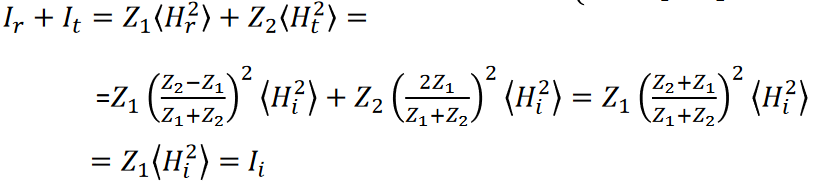
\includegraphics[width=0.5\textwidth]{screenshots/2024-05-07-11-55-08.png}
\end{figure}
Posso definire ancora i coefficienti di trasmissione e di riflessione:
\begin{definition}
	[Coefficienti di trasmissione e di riflessione]
	\begin{align}
		T &= \frac{4 Z_1 Z_2}{(Z_1 + Z_2)}^{2} &
		R &= \left( \frac{Z_2 - Z_1}{Z_1 + Z_2} \right)^{2}  
	\end{align}
	Per definizione \(R + T = 1\), \(I_t = T I_i\) e \(I_r = R I_i\).
\end{definition}